\documentclass[tikz,border=10pt]{standalone}
\usepackage{xcolor}

\definecolor{mainblue}{HTML}{001158}
\definecolor{accent}{HTML}{8592bc}
\definecolor{lightaccent}{HTML}{e7e9f2}

\begin{document}
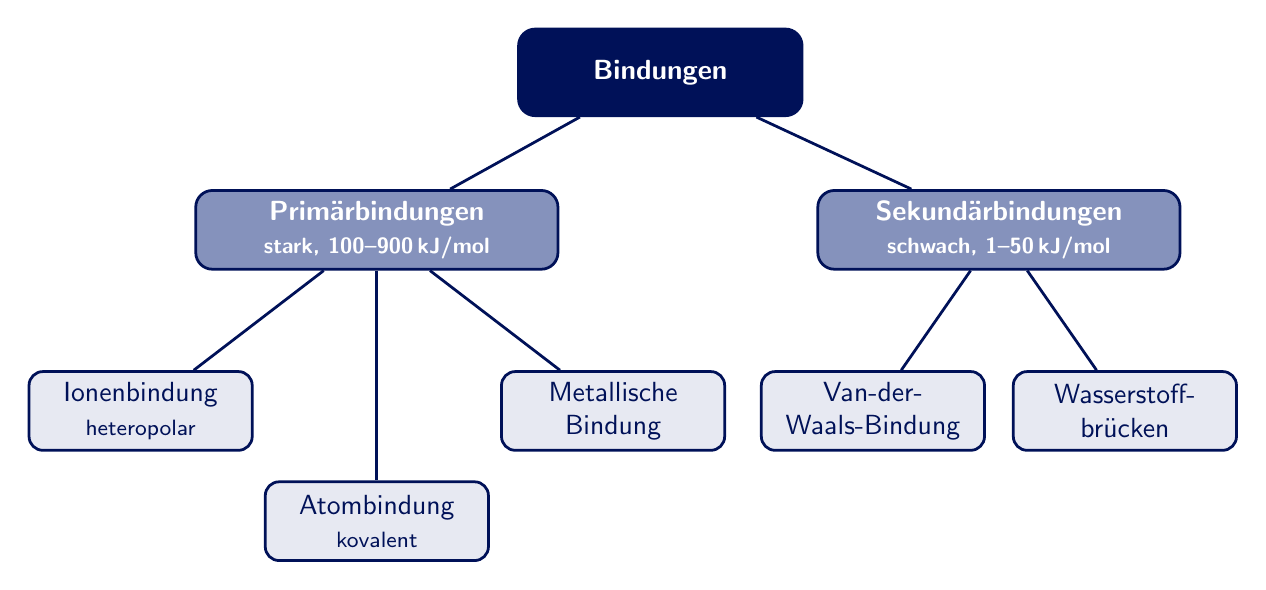
\begin{tikzpicture}[
    font=\sffamily,
    root/.style={
        rectangle, rounded corners=6pt, draw=mainblue, fill=mainblue, text=white,
        align=center, minimum width=3.6cm, minimum height=1.1cm, line width=1pt, font=\sffamily\bfseries
    },
    cat/.style={
        rectangle, rounded corners=6pt, draw=mainblue, fill=accent, text=white,
        align=center, minimum width=4.6cm, minimum height=1.0cm, line width=1pt, font=\sffamily\bfseries
    },
    leaf/.style={
        rectangle, rounded corners=5pt, draw=mainblue, fill=lightaccent, text=mainblue,
        align=center, text width=2.6cm, minimum height=1.0cm, line width=1pt, font=\sffamily
    },
    edge/.style={draw=mainblue, line width=1pt}
]

\node[root] (root) at (0,4.3) {Bindungen};

\node[cat] (prim) at (-3.6,2.3) {Prim\"arbindungen\\\footnotesize stark, 100--900\,kJ/mol};
\node[cat] (sek)  at (4.3,2.3)  {Sekund\"arbindungen\\\footnotesize schwach, 1--50\,kJ/mol};

\draw[edge] (root) -- (prim);
\draw[edge] (root) -- (sek);

\node[leaf] (ion) at (-6.6,0) {Ionenbindung\\\footnotesize heteropolar};
\node[leaf] (kov) at (-3.6,-1.4) {Atombindung\\\footnotesize kovalent};
\node[leaf] (met) at (-0.6,0) {Metallische\\Bindung};

\draw[edge] (prim) -- (ion);
\draw[edge] (prim) -- (kov);
\draw[edge] (prim) -- (met);

\node[leaf] (vdw) at (2.7,0) {Van-der-\\Waals-Bindung};
\node[leaf] (hbr) at (5.9,0) {Wasserstoff-\\br\"ucken};

\draw[edge] (sek) -- (vdw);
\draw[edge] (sek) -- (hbr);

\end{tikzpicture}
\end{document}
